\documentclass[a4paper,titlepage,12pt,twoside,openright]{scrreprt}

\usepackage{fancyref}
\usepackage{multirow}
\usepackage{tikz}
\usetikzlibrary{trees}
\usetikzlibrary{shapes}
\usepackage{listings}

% Include style for title page, legal clause, and required classes.
% Also sets the page style, header and footer.
\usepackage{cappstyle}

% Enter your hyphenation list, i.e. hy-phe-na-tion, in order to have these
% words hyphenated correctly at the end of a line. Use spaces to separate 
% words.
\hyphenation{}

\begin{document}

	% make empty pages clear without any header, without any footer
    \pagestyle{empty}

    \capptitle{Studienarbeit}
         {}                         % nuber of this thesis, normally blank
         {Fast~and~Exact~Floating-Point~Accumulation}  % title of thesis
         {Reimar~D�ffinger}                % author name
         {Dr.~Rainer~Buchty} % supervisor
         {M�rz 2008}        % month & year (for title page)
         {Reimar D�ffinger\\ 
          Schauinslandstr. 4\\ 
          75249 Kieselbronn\\ 
          email: Reimar.Doeffinger@gmx.de}     % address
          {Prof.~Dr.~Wolfgang~Karl}
          
    \cappclause{Reimar D�ffinger}          % author name
         {Karlsruhe, 01.03.2008}    % location, date (for legal clause)


    % reset parskip to more useful settings than 1.5ex as in cappstyle.sty
    \setlength{\parskip}{1.45ex plus 0.5ex minus 0.2ex}

    \cleardoublepage
    % Abstract
    \begin{abstract}
  \begin{center}
    \textbf{\abstractname}
  \end{center}
\end{abstract}

    \cleardoublepage

    \pagenumbering{Roman}
    \pagestyle{plain}
    \tableofcontents
    \listoftables
    \listoffigures
    \cleardoublepage

	\pagestyle{myfancy}
    % include this numbering in this file as it does not work when directly 
% including in Dokument.tex
\pagenumbering{arabic}

\chapter{Motivation}
It is well known that the ever increasing computing speed allows more
and more problems to be solved computationally.
But it also means --- especially with iterative algorithms --- that problems
that could already be solved before can now be solved with higher accuracy.
Thus, calculations can now much more easily hit the accuracy limit of the
computer's native number format --- usually IEEE 754 double precision floating
point.
There are several solutions to this. One is to just increase the size of the
floating point format once again, as when switching from single- to
double-precision (a switch, that in case of Cell or GPU processing is still in
progress).
Another is full software emulation of larger data types as e.g. the
MPFR library~\footnote{\url{http://www.mpfr.org}} provides.\\
The approach used here instead is based on the previous work by
Dr. Ulrich W. Kulisch~\cite{advar} and --- while keeping the current native
floating point numbers --- implements additional, exact operations on these.
Compared to just increasing the size of floating point numbers this has the
advantage that at least some operations will be exact, and thus there is no
need for an error estimation on these, which is a big advantage since error
estimation is difficult and imprecise when done on a theoretical level
beforehand and slow and often still imprecise when done during runtime e.g.
via interval arithmetic.
Compared to a full software implementation it is still very well implementable
in hardware, thus allowing for much faster speed.\\
In the following, only an exact accumulation operation on single precision floating
point numbers and its implementation is presented.\\
Extending the design to support double precision should be a question of solving
some minor, but time consuming technical issues due to e.g. HyperTransport data
unit size being only 32 bit.\\
Contrary to the work by Dr. Kulisch, multiplication was not implemented since
multipliers on FPGAs especially for large sizes can simply not compete with
those in a modern CPU and would use up a lot of hardware resources even if
a user might have more use for e.g. square-root-and-accumulate than
multiply-and-accumulate.



    \chapter{Basic HyperTransport Concepts}

To ease understanding of some of the implementation approaches, I will describe
some of the basics of HyperTransport and some of the details that are not easy
find elsewhere.\\
For more details and precise descriptions, please refer to the HyperTransport
specification~\cite{htspec}.\\
HyperTransport is a high-speed device interconnect, used in particular by AMD CPUs.
A HyperTransport link always connects exactly two devices, which means reduced
management overhead compared to and ordinary bus, while still allowing to connect many
devices by allowing chaining of links, tunnels and bridges.\\
An optional part of the specification also allows for more complex HyperTransport
networks with more advanced routing.\\
On the physical level, HyperTransport uses differential signalling and independent links
for each communication direction.\\
Link speed can be varied independently in each direction as well, allowing any combination
of link frequencies from 200 to 2600 MHz (DDR) and link widths of 2 bits to 32 bits (requiring
29 to 199 pins respectively~\cite{htarch}).\\
Each link also uses 3 independent virtual channels (i.e. each has their own buffers so
they can not block each other): posted, nonposted and response.\\
Flow control is done using a credit-based system: each virtual channel has an
associated number of credits on the sender side (representing available buffers on
the receiver side), independent for command and data.\\
Sending a command/data reduces the number of credits on the sender side,
the receiver increases them again by sending appropriate nop command packets
(nops do not use credits, thus no deadlocks are possible).\\
For data, each data packet uses one credit (size can vary between 4 and 64 bytes).
There is an optional data credit mode where each 4 bytes of data use up one
credit, but this is not available in the implementation used.\\
The implementation used provides 32 credits for each virtual channel, for both
command and data.\\
HyperTransport devices are configured (e.g. base address) by a set of registers
with same layout and behaviour as PCI configuration registers, so it is easily
possible to use a HyperTransport device just like a PCI device, just with a much
faster and lower latency connection.\\




Credits for commands are restored to the sender automatically when they are
read from the fifo, whereas for data (since it can have varying size) an
explicit data\_complete signal must be used.\\
Since correct handling of this signal increases complexity significantly
and wrong handling can result in the CPU hanging, this together with some
additional simplifications is handled separately in the ht\_simplify module.



    \chapter{Components of the Hardware Design}

\begin{center}
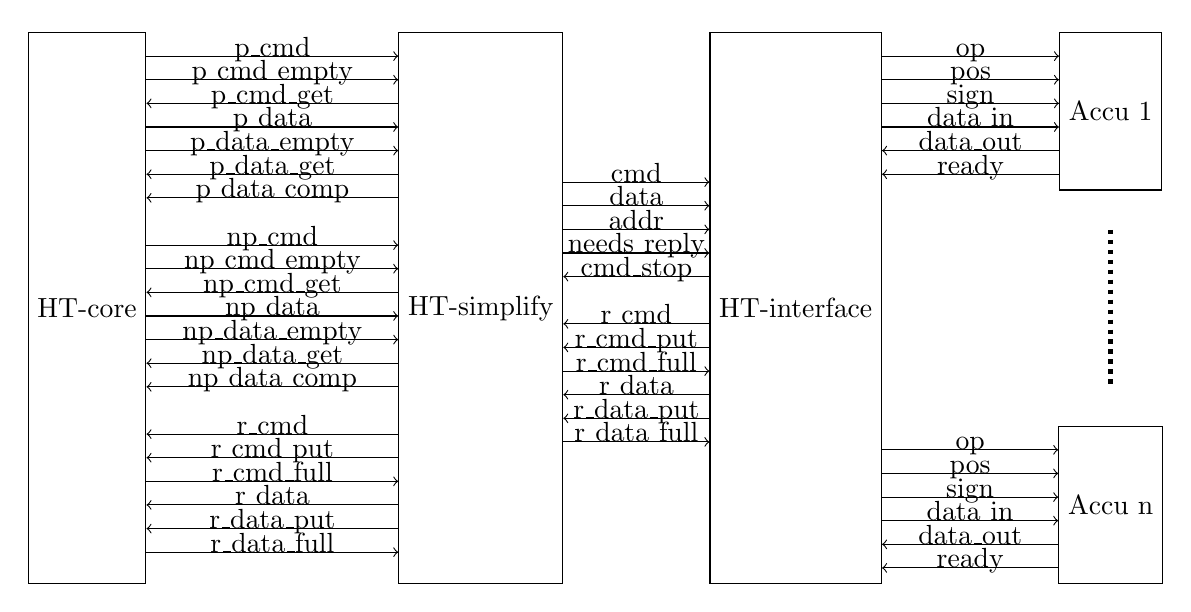
\begin{tikzpicture}
  \tikzstyle{every node}=[rectangle,draw]
  \node[minimum height=7cm] (HT-core)      at (0   ,0) {HT-core};
  \node[minimum height=7cm] (HT-simplify)  at (50mm,0) {HT-simplify};
  \node[minimum height=7cm] (HT-interface) at (90mm,0) {HT-interface};
  \node[minimum height=2cm] (acc1) at (130mm,+25mm) {Accu 1};
  \node[minimum height=2cm] (accn) at (130mm,-25mm) {Accu n};
  \tikzstyle{dots}=[dotted,ultra thick]
  \draw[dots,shorten >=5mm,shorten <=5mm] (acc1) -- (accn);

%% draw connections
  \tikzstyle{every node}=[pos=0.5,draw=none,anchor=base]

%% core <-> simplifier connections
  \newcommand{\mysc}{-3mm}
  \newcommand{\myofs}{32mm}
  \foreach \n/\txt in {  0/p\_cmd,   1/p\_cmd\_empty,   3/p\_data,   4/p\_data\_empty,
                         8/np\_cmd,  9/np\_cmd\_empty, 11/np\_data, 12/np\_data\_empty,
                        18/r\_cmd\_full, 21/r\_data\_full}
    \draw[->] ([yshift=\mysc*\n+\myofs] HT-core.east) -- ([yshift=\mysc*\n+\myofs] HT-simplify.west) node {\txt};
  \foreach \n/\txt in {  2/p\_cmd\_get,   5/p\_data\_get,   6/p\_data\_comp,
                        10/np\_cmd\_get, 13/np\_data\_get, 14/np\_data\_comp,
                        16/r\_cmd,       17/r\_cmd\_put,   19/r\_data,        20/r\_data\_put}
    \draw[<-] ([yshift=\mysc*\n+\myofs] HT-core.east) -- ([yshift=\mysc*\n+\myofs] HT-simplify.west) node {\txt};

%% simplifier <-> mmap interface connections
  \renewcommand{\mysc}{-3mm}
  \renewcommand{\myofs}{16mm}
  \foreach \n/\txt in {  0/cmd, 1/data, 2/addr, 3/needs\_reply,
                         8/r\_cmd\_full, 11/r\_data\_full}
    \draw[->] ([yshift=\mysc*\n+\myofs] HT-simplify.east) -- ([yshift=\mysc*\n+\myofs] HT-interface.west) node {\txt};
  \foreach \n/\txt in {  4/cmd\_stop,
                         6/r\_cmd,        7/r\_cmd\_put,    9/r\_data,        10/r\_data\_put}
    \draw[<-] ([yshift=\mysc*\n+\myofs] HT-simplify.east) -- ([yshift=\mysc*\n+\myofs] HT-interface.west) node {\txt};

%% mmap interface <-> accumulators connections
  \renewcommand{\mysc}{-3mm}
  \renewcommand{\myofs}{7mm}
  \foreach \n/\txt in {  0/op, 1/pos, 2/sign, 3/data\_in} {
    \draw[->] ([yshift= 25mm+\mysc*\n+\myofs] HT-interface.east) -- ([yshift=\mysc*\n+\myofs] acc1.west) node {\txt};
    \draw[->] ([yshift=-25mm+\mysc*\n+\myofs] HT-interface.east) -- ([yshift=\mysc*\n+\myofs] accn.west) node {\txt};
  };
  \foreach \n/\txt in {  4/data\_out, 5/ready} {
    \draw[<-] ([yshift= 25mm+\mysc*\n+\myofs] HT-interface.east) -- ([yshift=\mysc*\n+\myofs] acc1.west) node {\txt};
    \draw[<-] ([yshift=-25mm+\mysc*\n+\myofs] HT-interface.east) -- ([yshift=\mysc*\n+\myofs] accn.west) node {\txt};
  };
\end{tikzpicture}.

\end{center}

\section{The HyperTransport Core}

The HyperTransport implementation used is the "HT Core" by the Computer
Architecture Group of the University of Mannheim, more specifially the
version 0.9 for 16-bit links from September 2007.\\
This implementation handles HyperTransport data credits in a non-trivial
way, and since its documentation does not explain this clearly, it is
explained here.\\
Credits for commands are restored to the sender automatically when they are
read from the fifo, whereas for data (since it can have varying size) an
explicit data\_complete signal must be used.\\
This signal must be set to high for exactly one cycle each time a data packet
has been completely read. In particular, it must not be set if a command
has no associated data, and it must be set for only one cycle even if reading
all associated data takes multiple cycles, and it must be set after or
exactly when the last data of the packet is shifted out of the FIFO.\\
Since correct handling of this signal increases complexity significantly
and wrong handling can result in the CPU hanging, this together with some
additional simplifications is handled separately in the ht\_simplify module,
described in~\fref{sec:htsimplify}.

\section{The HyperTransport Simplification Layer}
\label{sec:htsimplify}

The HyperTransport simplification layer (the module called ht\_simplify)
merges the posted and non-posted queue into one queue, handles setting
the data\_complete signals of the HyperTransport core, splits multi-dword
writes into multiple writes of a single dword and inserts nop
commands into the queue as necessary, thus eliminating the need for
and extra "empty" signal, and provides a signal that indicates
if the current command must be replied to via the response queue.\\
This greatly reduces the complexity and frustration of designing a device
that uses HyperTransport by handling the parts that are most error-prone
and easily lead to a stopped CPU.\\
In the current implementation it has also several drawbacks: byte-sized
writes are not handled correctly, and the transfer rate is limited to one command
and 32 bits data per clock cycle, whereas the HT Core allows for up to one
command and 64 bits of data per clock cycle per queue.\\

\section{The Memory-Mapping Interface}
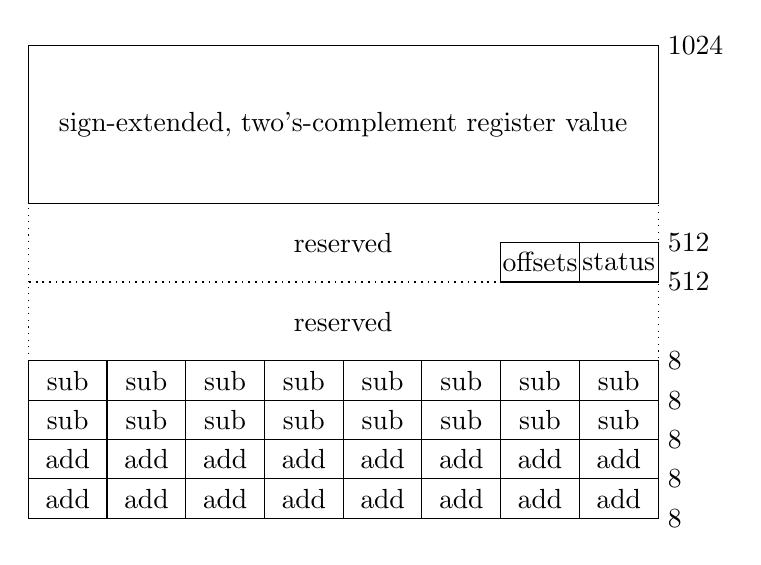
\begin{tikzpicture}
  \newcommand{\rectw}{10mm}
  \newcommand{\recth}{5mm}
  \newcommand\drawblock[3]{\draw (#1*\rectw,#2*\recth) rectangle +(\rectw,\recth);\draw (#1*\rectw+\rectw/2,#2*\recth+\recth/2) node {#3};}
  \newcounter{addr}
  \foreach \y/\text in {0/add,1/add,2/sub,3/sub}{
    \setcounter{addr}{8*\y}
    \draw (8*\rectw,\y*\recth) node[right] {\arabic{addr}};
    \foreach \x in {0,...,7}{
      \drawblock{\x}{\y}{\text}
    }
  }
  \setcounter{addr}{8*4}
  \draw (8*\rectw,4*\recth) node[right] {\arabic{addr}};

% reserved command part
  \draw[style=dotted] (0*\rectw,4*\recth) rectangle +(8*\rectw,2*\recth);
  \draw (4*\rectw,5*\recth) node {reserved};

  \draw (8*\rectw,6*\recth) node[right] {512};
% status flags/offsets part
  \drawblock{7}{6}{status}
  \drawblock{6}{6}{offsets}
  \setcounter{addr}{512+8}
  \draw (8*\rectw,7*\recth) node[right] {\arabic{addr}};

% reserved status part
  \draw[style=dotted] (0*\rectw,6*\recth) rectangle +(8*\rectw,2*\recth);
  \draw (4*\rectw,7*\recth) node {reserved};

% main register
  \draw (0*\rectw,8*\recth) rectangle +(8*\rectw,4*\recth);
  \draw (4*\rectw,10*\recth) node {sign-extended, two's-complement register value};
  \draw (8*\rectw,12*\recth) node[right] {1024};

\end{tikzpicture}


    \chapter{The ALU core}
\section{Interface of the Accumulator VHDL Entity}
\newcommand\tabhead[1]{\hline\multicolumn{2}{|c|}{#1}\\ \hline}
\newcommand\tabline[2]{#1 & #2\\ \hline}
\begin{table}[htbp]
\begin{tabular}{|l|p{0.75\textwidth}|}
\tabhead     {Basic input signals}
\tabline {clock}     {sensitive to rising edge.}
\tabline {reset}     {set to 1 for an (asynchronous) reset.}
\hline
\tabhead     {Control input signals}
\tabline {sign}      {set to 1 for subtraction instead of addition (flip sign).}
\tabline {op}        {operation to execute. Use one of the op\_ constants.}
\tabline {data\_in}  {data to operate on.}
\tabline {pos}       {block position as signed value needed for some operations.}
\hline
\tabhead     {Output signals}
\tabline {ready}     {
        if 1 indicates that the operation given by the control input signals
        is now being processed and the control input signals should be set to
        the right values for the next operation.
        Use op\_nop if you do not have any next operation to execute (yet).
        The input signals may be changed at any time, not only when ready
        is 1, any value when ready was not 1 will be ignored.}
\tabline {data\_out} {
        result data after any read operation. This will be valid the
        cycle after the ready signal becomes 1 to indicate the start of
        processing for the operation following the read.}
\end{tabular}
\caption{Ports of the ALU core}
\end{table}

\begin{table}
\begin{tabular}{|l|p{0.75\textwidth}|}
\hline
\tabline {Name}  {Function}
\hline
\tabline {op\_nop} {no operation, idle}
\tabline {op\_add} {
    add/subtract (depending on sign signal) a 64 bit block
    (representing a positive integer) at the 32 bit block offset
    specified by the pos signal.}
\tabline {op\_readblock} {
    read 32 bit block specified by the pos signal, reads
    below the actually RAM-backed memory range return 0,
    reads above 0 for positive, X"FFFFFFFF" for negative values.}
\tabline {op\_writeblock} {
    write 32 bit block specified by the pos signal, writes outside
    the implemented range are ignored (ideally they should set overflow/
    underflow flags as appropriate).}
\tabline {op\_readflags} {
    read virtual 32 bit flag register. The upper 16 bits indicate
    which of the lower 16 bits (the actual flags) are valid.}
\tabline {op\_writeflags} {
    set the flags marked by a set bit in the upper 16 bits to
    the value in the lower 16 bits.
    This is mostly for allowing to restore the register state from system
    RAM and rarely useful otherwise.}
\tabline {op\_readoffsets} {
    get exponent offsets for floating point operations.
    Exponent offsets are two 16 bit signed integers.
    Lower 16 bits are for writes (op\_floatadd) higher 16 bits for reads (op\_readfloat).}
\tabline {op\_writeoffsets} {
    set exponent offsets for floating point operations.
    Exponent offsets are two 16 bit signed integers.
    Lower 16 bits are for writes (op\_floatadd) higher 16 bits for reads (op\_readfloat).}
\tabline {op\_readfloat} {
    reads the current register content as a single-precision
    floating-point value. Denormals and +/-Inf are supported, values that should
    be NaN are returned as +/-Inf.
    The pos signal is misused to specify the rounding mode, see~\fref{tab:round}.}
\tabline {op\_floatadd} {
    adds/subtracts (depending on sign signal) the given
    single-precision floating-point value. Note that NaN is treated as Inf
    currently.}
\end{tabular}
\caption{Operations of the ALU core}
\end{table}

\begin{table}
\begin{tabular}{|l|l|}
\hline
\tabline {pos signal} {rounding mode}
\hline
\tabline {0}          {round to $0$}
\tabline {1}          {round away from $0$}
\tabline {2}          {round to $-\infty$}
\tabline {3}          {round to $+\infty$}
\tabline {4}          {round to nearest}
\tabline {other}      {unspecified}
\end{tabular}
\caption{Rounding Modes}
\label{tab:round}
\end{table}

\section{Implementation details}
\subsection{Steps of the op\_floatadd Operation}

\renewcommand\tabline[2]{#1 & \multicolumn{5}{p{0.75\textwidth}|}{#2}\\}
\begin{tabular}{|r|p{0.25\textwidth}|r|p{0.25\textwidth}|r|p{0.25\textwidth}|}
\hline
\tabline {  0} {Handle Inf/NaN special cases by setting the overflow bit}
\tabline {  1} {combine sign of value with sign signal}
\tabline {  2} {extract 32 bit block position and shift value from exponent}
\tabline {  3} {extract mantissa (with leading 1 or 0 depending on denormal or not)}
\tabline {  4} {shift mantissa for alignment with 32 bit block boundary}
\tabline {  5} {load first 32 bit block}
\tabline {  6} {add/subtract lower part of mantissa to block value}
\tabline {  7} {store first 32 bit block}
\tabline {  8} {load second 32 bit block}
\tabline {  9} {add/subtract upper part of mantissa and carry to block value}
\tabline { 10} {store second 32 bit block}
\hline\hline
\multicolumn{6}{|p{0.75\textwidth}|}{
    The following steps are only necessary if carry is set,
    but currently they are done always to simplify the implementation}\\
\hline\hline
\tabline { 11} {calculate carry resolution position}
\tabline { 12} {flip bits in-between current position and carry-resolution position}
\hline
13a & load 32 bit block for carry resolution &
\multirow{3}{*}{13b} & \multirow{3}{0.25\textwidth}{flip sign bit as part of carry resolution} &
\multirow{3}{*}{13c} & \multirow{3}{0.25\textwidth}{set overflow bit as part of carry "resolution"}\\
14a & add/subtract carry & & & &\\
15a & store 32 bit block for carry resolution & & & &\\
\hline
\end{tabular}

These steps are organized into clock cycles as follows:
Clock 1: 0) - 3)
Clock 2: 4), 5)
Clock 3: 6), 8), 11), pre-calculate 12)
Clock 4: 7), 9), 13a)
Clock 5: 10), 12), 14a), 13b), 13c)
Clock 6: 15a)

Note that processing of the next operation starts with Clock 5, so in
each 4 cycles one floatadd operation can complete.
Reducing the number of clock cycles is difficult for several reasons:
1) Skipping carry resolution if there is no carry is probably easiest, but
   will increase code complexity since the carry value is only known after
   Clock 4, but to gain anything processing of the next instruction would
   have to start \em at \rm Clock 4.
2) The dual-port BlockRAM resource can not service more read-write requests
   than the current implementation uses, thus any improvements either need
   to use multiple BlockRAMs (which in a previous implementation resulted in
   low clock speeds) or a RAM resource with more than 2 ports.
3) Pipelining will need difficult dependency resolution, since the 32 bit blocks
   that are changed only become known for certain in step 12, though for the
   general case a worst-case guess based on the pre-calculated value for step
   12) may be good enough.

\subsection{Steps of the op\_readfloat Operation}

 1) Determine block number of highest set bit (highest bit not equal to sign),
    or the number of the block containing the lowest bit representable by a
    denormal if this is higher.
 2) read block determined in step 1 and the one below.
 3) determine position of first set/unset bit in read block.
 4) calculate exponent value with information from step 1) and 3).
 5) use value from step 3) to shift the blocks read in 2) so that the highest
    bit unequal to the sign is "leftmost".
 6) determine which is the lowest block that is not all 0.
 7) use results of steps 5) and 6) to check if the value can be represented
    exactly as float (special case for denormals, needs exponent from step 4).
 8) for negative values now invert the value from 5) (together with rounding
    converts two's complement to absolute value for mantissa).
 9) apply rounding if necessary (needs result from step 7 to avoid bias).
10) adjust exponent for possible carry due to rounding.
11) use sign, exponent from 10) and mantissa from 9) to build the float value.
    Needs special-case for denormals and infinities.

These steps are organized into clock cycles as follows:
Clock 1: wait, since this could overlap with calculation from previous operation
Clock 1a: wait if a write-back from a previous operation is pending
Clock 2: 1)
Clock 3: 2), 6)
Clock 4: 2), 3)
Clock 5: 4)
Clock 6: 4), 5), 7), 8)
Clock 7: 9), 10), 11)

\subsection{State machine}
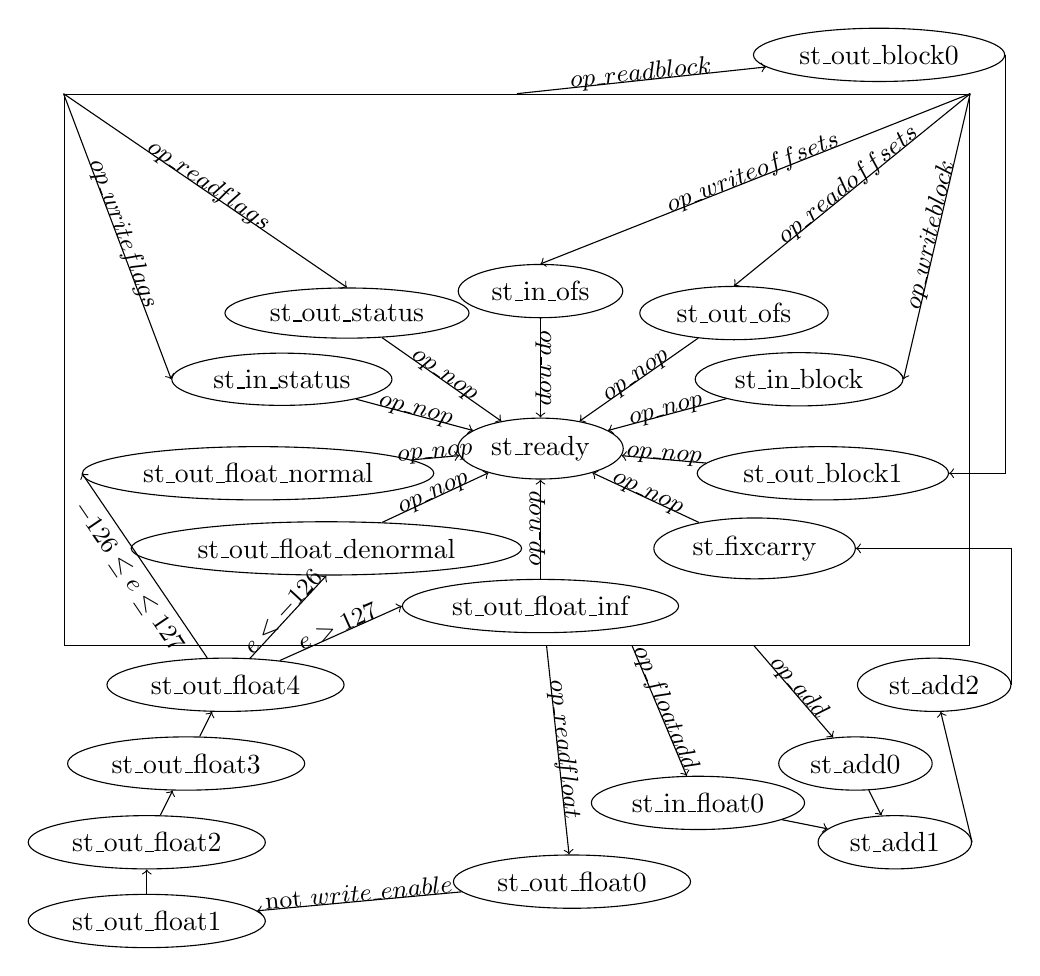
\begin{tikzpicture}
  \tikzstyle{every node}=[draw,shape=ellipse]
  \tikzstyle{op}=[midway,draw=none,sloped,anchor=base]
  \node[shape=rectangle, minimum width=11.5cm, minimum height=7cm] (finals) at (-3mm,1cm) {};
  \newcommand{\dist}{2cm}
  \node (ready)              at (0cm, 0mm)     {st\_ready};
  \node (fixcarry)           at (-25:30mm)     {st\_fixcarry};
  \node (out_block1)         at ( -5:36mm)     {st\_out\_block1};
  \node (in_block)           at ( 15:34mm)     {st\_in\_block};
  \node (out_ofs)            at ( 35:30mm)     {st\_out\_ofs};
  \node (in_ofs)             at ( 90:20mm)     {st\_in\_ofs};
  \node (out_status)         at (145:30mm)     {st\_out\_status};
  \node (in_status)          at (165:34mm)     {st\_in\_status};
  \node (out_float_normal)   at (185:36mm)     {st\_out\_float\_normal};
  \node (out_float_denormal) at (205:30mm)     {st\_out\_float\_denormal};
  \node (out_float_inf)      at (270:20mm)     {st\_out\_float\_inf};
  \foreach \src in {fixcarry,out_block1,in_block,out_ofs,in_ofs,out_status,in_status,
                    out_float_normal,out_float_denormal,out_float_inf}{
    \draw[->] (\src) -- (ready)                node[op] {\small $op\_nop$};
  }
% state transitions inside "final" states
  \draw[->] (finals.north east) -- (in_block.east)        node[op] {\small $op\_writeblock$};
  \draw[->] (finals.north east) -- (out_ofs.north)        node[op] {\small $op\_readoffsets$};
  \draw[->] (finals.north east) -- (in_ofs.north)         node[op] {\small $op\_writeoffsets$};
  \draw[->] (finals.north west) -- (out_status.north)     node[op] {\small $op\_readflags$};
  \draw[->] (finals.north west) -- (in_status.west)       node[op] {\small $op\_writeflags$};
% non-"final" states and transitions
  \node (out_block0)         at ( 43mm, 50mm)  {st\_out\_block0};
  \draw[->] (finals.north) -- (out_block0)     node[op] {\small $op\_readblock$};
  \draw[->] (out_block0.east) |- (out_block1);
  \node (add0)               at ( 40mm,-40mm)  {st\_add0};
  \draw[->] (finals) -- (add0)                 node[op] {\small $op\_add$};
  \node (in_float0)          at ( 20mm,-45mm)  {st\_in\_float0};
  \draw[->] (finals) -- (in_float0)            node[op] {\small $op\_floatadd$};
  \node (add1)               at ( 45mm,-50mm)  {st\_add1};
  \draw[->] (add0) -- (add1);
  \draw[->] (in_float0) -- (add1);
  \node (add2)               at ( 50mm,-30mm)  {st\_add2};
  \draw[->] (add1.east) -- (add2);
  \draw[->] (add2.east) |- (fixcarry);
  \node (out_float0)         at (  4mm,-55mm)  {st\_out\_float0};
  \node (out_float1)         at (-50mm,-60mm)  {st\_out\_float1};
  \node (out_float2)         at (-50mm,-50mm)  {st\_out\_float2};
  \node (out_float3)         at (-45mm,-40mm)  {st\_out\_float3};
  \node (out_float4)         at (-40mm,-30mm)  {st\_out\_float4};
  \draw[->] (finals) -- (out_float0)           node[op] {\small $op\_readfloat$};
  \draw[->] (out_float0) -- (out_float1)       node[op] {\small not $write\_enable$};
  \draw[->] (out_float1) -- (out_float2);
  \draw[->] (out_float2) -- (out_float3);
  \draw[->] (out_float3) -- (out_float4);
  \draw[->] (out_float4) -- (out_float_normal.west) node[op,below=-1mm] {\small $-126 \le e \le 127$};
  \draw[->] (out_float4) -- (out_float_denormal.south) node[op] {\small $e < -126$};
  \draw[->] (out_float4) -- (out_float_inf.west) node[op] {\small $e > 127$};
\end{tikzpicture}




    Meaning of the flags:
    Bit 0: sign
    Bit 1: overflow
    Bit 2: zero

    Meaning of the bit values:
    Bit 0: sign (only the sign is set, the value stored in the RAM is not
           changed. There is probably no practical use for this).
    Bit 1: overflow. Periodically checking and clearing the overflow flag
           can be used to detect ranges of summands that contain Inf or NaN
           and may need additional, more careful processing later.
    Bit 2: zero. Setting to 0 has no effect, setting to 1 clears the register
           (bits 0 and 1 should be set to 0 at the same time preferably).

    \newcommand*{\fancyreflstlabelprefix}{lst}
\frefformat{vario}{\fancyreflstlabelprefix}{listing\fancyrefdefaultspacing#1#3}
\Frefformat{vario}{\fancyreflstlabelprefix}{Listing\fancyrefdefaultspacing#1#3}
\lstdefinelanguage[x86att]{Assembler}{
  morekeywords={
    add, addl, addq, call, clflush, enter, jmp, leave,
    mov, movaps, movl, movslq, movss, movq,
    pop, popl, push, pushl, ret, sal, sall, sub, subl, xor, xorl
  },
  morecomment=[l];,
  morecomment=[l]\#,
  morestring=[b]",
  morestring=[b]',
  keywordsprefix=\%
}

\lstset{basicstyle=\ttfamily}
\lstset{breaklines=true}
\lstset{captionpos=b,columns=[c]flexible}
\lstset{language=C}

\chapter{The Software Interface}
For accessing the hardware a simple C library interface is provided.
\Fref{lst:efacexample} is a small example program showing the basic
use of this library, derived from one of the test programs for the design.
\lstinputlisting[caption=example code for libefac use,label=lst:efacexample]{examplesum.c}
\section{Available Functions}
\section{Optimization Tricks}
This section will explain some of the very specific tricks used in
order to generate faster and smaller code to access the device.
They are not very useful yet, since the speed of the device itself
is the major limit and no software optimizations help (though smaller
code always means less cache pressure).
Still these details may be interesting to some and should help
understand the code.\\
The following explanations assume at least basic knowledge of x86
assembler and how application linking and operating systems work.\\
For a reference of x86 assembler instructions refer to e.g. AMD's
Programmer's Manuals~\cite{amdinstr}.\\
To demonstrate these various tricks, the code in~\fref{lst:demo}
is compiled in several different ways.\\
All tests were done with "gcc (GCC) 4.1.2 (Ubuntu 4.1.2-0ubuntu4)",
and unless indicate otherwise were build for the x86\_64 architecture.\\
In these examples, the device address range is assumed to be marked
uncacheable which might not be the best option for optimal speed but
simplifies the code for demonstration --- the difference is just a
missing instruction like clflush or mfence.\\


\begin{lstlisting}[float=ht,caption=compilation demonstration code,label=lst:demo]
#include "libefac.h"
void test(void) {
  efac_add4(0, 1.0, 1.0, 1.0, 1.0);
}
\end{lstlisting}

\lstset{language={[x86att]Assembler}}

The C library during efac\_init maps the physical address space of the
device into the application's address space. This is done via mmap,
and usually the choice of virtual address is left to mmap and the
resulting address stored in a variable.\\
This leads to assembler code as in~\fref{lst:regptr}. efac\_regs
here is a pointer variable (declared as "uint32\_t *efac\_regs").
The contents of this pointer variable as a first step must be loaded
into a register.\\
If now efac\_regs is instead declared as an array
("uint32\_t efac\_regs[REGISTER\_SIZE]") and the device simply mapped
"over" it, the address is already known at link time and can be hard-code,
as~\fref{lst:inline64} shows. Note that this trick may fail if compiling
a dynamic library (more precisely if generating position-independent code).\\

\begin{lstlisting}[float=ht,caption={x86\_64 using register pointer (gcc -S -m64 -O3)},label={lst:regptr}]
test:
        movq    efac_regs(%rip), %rdx
        movl    $0x3f800000, %eax
        movl    %eax, 64(%rdx)
        movl    %eax, 68(%rdx)
        movl    %eax, 72(%rdx)
        movl    %eax, 76(%rdx)
        ret
\end{lstlisting}

\begin{lstlisting}[float=ht,caption={x86\_64 inlined (gcc -S -m64 -O3)},label={lst:inline64}]
test:
        movl    $0x3f800000, %eax
        movl    %eax, efac_regs+64(%rip)
        movl    %eax, efac_regs+68(%rip)
        movl    %eax, efac_regs+72(%rip)
        movl    %eax, efac_regs+76(%rip)
        ret
\end{lstlisting}

Another optimization is that except for initialization most of the code is
in the header file, so that the functions can be inlined. The benefit is
not only that the function call overhead is saved, but also expressions
based on constant function arguments can be calculated at compile-time
instead of runtime.\\
In \fref{lst:noinline64} the address must be calculated at runtime,
whereas due to inlining the can be calculated at compile-time in
\fref{lst:inline64}. Of course this pre-calculation is only possible
if the register number is a constant, but this should be the much
more common case --- on most CPU architectures the register number
is coded into the instruction at compile-time as well.\\
Note that the effect of inlining is even more pronounced when compiling
for 32 bit x86 architecture, as a comparison between \fref{lst:inline32}
and \fref{lst:noinline32} shows. This is because the 32 bit ABI passes
all arguments via the stack, which means the function needs a stack
frame and the data must be loaded from stack into a register before
it can be written again to the device.\\


\begin{lstlisting}[float=ht,caption={x86\_64 not inlined (gcc -S -m64 -O3 -fno-inline)},label={lst:noinline64}]
efac_add4:
        sall    $12, %edi
        movslq  %edi,%rdi
        addq    $efac_regs, %rdi
        movss   %xmm0, 64(%rdi)
        movss   %xmm1, 68(%rdi)
        movss   %xmm2, 72(%rdi)
        movss   %xmm3, 76(%rdi)
        ret

test:
        movss   .LC0(%rip), %xmm3
        xorl    %edi, %edi
        movaps  %xmm3, %xmm2
        movaps  %xmm3, %xmm1
        movaps  %xmm3, %xmm0
        jmp     efac_add4
\end{lstlisting}

\begin{lstlisting}[float=ht,caption={x86 inlined (gcc -S -m32 -O3)},label={lst:inline32}]
test:
        movl    $0x3f800000, %eax
        pushl   %ebp
        movl    %esp, %ebp
        movl    %eax, efac_regs+64
        movl    %eax, efac_regs+68
        movl    %eax, efac_regs+72
        movl    %eax, efac_regs+76
        popl    %ebp
        ret
\end{lstlisting}

\begin{lstlisting}[float=ht,caption={x86 not inlined (gcc -S -m32 -O3 -fno-inline)},label={lst:noinline32}]
efac_add4:
        pushl   %ebp
        movl    %esp, %ebp
        movl    8(%ebp), %edx
        sall    $12, %eax
        addl    $efac_regs, %eax
        movl    %edx, 64(%eax)
        movl    12(%ebp), %edx
        movl    %edx, 68(%eax)
        movl    16(%ebp), %edx
        movl    %edx, 72(%eax)
        movl    20(%ebp), %edx
        movl    %edx, 76(%eax)
        popl    %ebp
        ret

test:
        pushl   %ebp
        movl    $0x3f800000, %eax
        movl    %esp, %ebp
        subl    $16, %esp
        movl    %eax, 12(%esp)
        movl    %eax, 8(%esp)
        movl    %eax, 4(%esp)
        movl    %eax, (%esp)
        xorl    %eax, %eax
        call    efac_add4
        leave
        ret
\end{lstlisting}


    \appendix

%    \input{doxygen/latex/refman}

    \nocite{*}
%     \bibliographystyle{geralpha}
    \bibliographystyle{plain}
    \bibliography{Bibliografie}


\end{document}
